
%(BEGIN_QUESTION)
% Copyright 2013, Tony R. Kuphaldt, released under the Creative Commons Attribution License (v 1.0)
% This means you may do almost anything with this work of mine, so long as you give me proper credit

Suppose an operator discovers that the natural gas make-up valve in this fuel gas pressure control system is shut when the controller output is 78\%.  A technician begins diagnosing the loop, following the steps shown (in order):

$$\includegraphics[width=15.5cm]{i0014rx01.eps}$$

\begin{itemize}
\item{} {\bf Test 1:} Measured 18.6 volts DC between PT-528 transmitter terminals.
\vskip 25pt
\item{} {\bf Test 2:} Measured supply air pressure at PV-528a to be 22 PSIG.
\vskip 25pt
\item{} {\bf Test 3:} Measured 0 volts DC between terminals 25 and 26.
\vskip 25pt
\item{} {\bf Test 4:} Measured 27 volts DC between terminals 5 and 6.
\vskip 25pt
\item{} {\bf Test 5:} Measured 27 volts DC between terminals 19 and 20.
\vskip 25pt
\item{} {\bf Test 6:} Measured 27 volts DC between terminals 15 and 16.
\vskip 25pt
\end{itemize}

Identify any useful information about the nature or location of the fault derived from the results of each test, in order of the tests performed.  If the test is not useful (i.e. provides no new information), mark it as such.  Assuming there is only one fault in the circuit, identify the location and nature of the fault as precisely as you can from the test results shown above.

\vfil 

\underbar{file i04792}
\eject
%(END_QUESTION)





%(BEGIN_ANSWER)

\begin{itemize}
\item{} {\bf Test 1:} Measured 18.6 volts DC between PT-528 transmitter terminals.  {\it Proves nothing that is helpful in diagnosing the valve problem.  We know the transmitter has adequate power to function, but this tells us nothing about why the make-up valve refuses to open.}
\vskip 5pt
\item{} {\bf Test 2:} Measured supply air pressure at PV-528a to be 22 PSIG.  {\it Proves that the air supply to the make-up valve is good (needs to be more than 15 PSI for a 3-15 PSI bench-set valve).  However, we don't know anything more about the fault other than the fact it isn't this one thing.}
\vskip 5pt
\item{} {\bf Test 3:} Measured 0 volts DC between terminals 25 and 26.  {\it Proves the fault is electrical in nature: either an ``open'' between these terminals and the DCS output, or a ``short'' potentially anywhere in this cable (or in the I/P) for valve PV-528a.}
\vskip 5pt
\item{} {\bf Test 4:} Measured 27 volts DC between terminals 5 and 6. {\it Proves the fault must be an ``open'' somewhere between these terminals and terminals 25-26.}
\vskip 5pt
\item{} {\bf Test 5:} Measured 27 volts DC between terminals 19 and 20. {\it This is an unnecessary test, as we already know there will be full voltage here, since points ``downstream'' of these (i.e. closer to the load) have full voltage.}
\vskip 5pt
\item{} {\bf Test 6:} Measured 27 volts DC between terminals 15 and 16. {\it Proves the fault must be an ``open'' between these terminals and terminals 25-26.}
\vskip 5pt
\end{itemize}

\vskip 10pt

{\bf The fault is an ``open'' in wire pair 5 of cable MOLSV-10, or at the connection point between one of these wires and the terminal block.}

%(END_ANSWER)





%(BEGIN_NOTES)


%INDEX% Troubleshooting review: electric circuit diagnostic test rationale

%(END_NOTES)


